\chapter{Acquisition of non-stationary impedance}
\minitoc

\section{Multi-frequency data acquisition}
The estimation of the impedance require the sampling of input and output signals from the system when an excitation signal is applied. For electrochemical systems, one uses an electrochemical workstation that contain all the hardware necessary to impose a desired voltage or current to the cell. In this work we exploit the possibility of an electrochemical workstation to recieve external signals and output the analog signals of voltage and current. This features is available for different brands, in my work I used a BioLogic device. This possibility has two advantages: generate an excitation signal of arbotrary complexity provided by dedicated high-end generator, and acquire the cell signals at very high frequency with dedicated device. This possibilities are not avalable using the softwar eprovided by the manifacturers. Usually no arbitrary signals can be used or they are very limited in the number of points and generation frequency, and secondly the maximum sampling frequency is low (5kHz at best). Fruthermore data can not be used for online caluclation using computation languages like Python. On the other hand the use of commercial electrochemical workstation lifts us from the work to develop custom electronic control suitable for high frequency and small currents. \\
\subsection{Description of the set-up}
For this work we assembled multiple set-ups using BioLogic electrochemical workstations, Keysight waveform generator and PicoTech Picoscope acquisition devices. The components are connected together using the auxiliary input-output port of the workstation. The waveform generator to the input (that superimpose the signals through an analog circuit) and the scope recieves the voltage and current signals for the synchronous sampling. The series and the model might vary experiment by experiment, therefore I will report the exact devices in the next part of the thesis where the results of discussion of multiple application of DEIS are reported. The brand, though, remain the same as well as the operating principles and software for their control that is the topic of the current chapter.\\
BioLogic workstations have for each channel an auxiliary 9-pin port for the input and output of analog signals. For the purpose of this project I was interested in only three: Input (Auciliary In2), voltage monitor and current monitor. The company supplies adapters for the 9-pin to BNC connectors but for me was more practical to just build them myself. A reference for the contruction is available in the appendix.\\
Appendix: Each channel of BioLogic workstation (not valid for cycler) has a 9-pin port adibits for input and output for the connection of external devices. The manual provides all the details on the pins positioning such that one can build their own cable. As material we gathered a 9-pin connector, BNC connector and coaxial cable. As instrumentation was needed only a solder with tin soldering wire and sharp scissors to cut and unsking the cable.\\
I needed to access the pins X, Y and Z, as in figure XX. I then used 3 cables, soldering the core to the proper pin and the shell together to the ground. Finally I connected the other end of the cable to the BNC connecter and close the encapsulation of the 9-pin connector after testing all the terminal points with a multimeter. Figure XX shows the soldering on the 9-pin connector.\\
End appendix\\
\section{Automation of the acquisition for batteries}
\subsection{Problem statement}
In the simplest scenerio, the acquisition of multi-frequency signals with the set-up explained above, requires only to use a programming language to manage the streaming of the signals from the oscilloscope to the computer and store them. The previous publication of the group exactly followed this idea. Specifically a MATLAB script was used (Github Battistell?). The MATLAB script was adapted from the examples provided by the manifacturer. For my project I made Python implementation beyond the simple script defining a practical object (a library) for a much compact code. The details of the Python implementation, and the design behind it are given in the Appendix. The potentiostat is used only for the electric control of the cell while not applying any perturbation (0V chronoamperometry or 0A chronopotentiometry) while the waveform generator provides the multi-frequency small excitation as well as the quasi-cyclic voltammetry pattern. The arbitrary waveforms are loaded manually to the device via a .arb file transferred via USB drive from the computer. How the .arb file is build?
This approach was the one I used for the first two applications (topic of the third and final part of the thesis) of the dynamic impedance for energy storage, also published as peer-review articles.\\
For the goal of the thesis of acquiring the dynamic impedance during the CCCV cycling of a battery the previously described approach is not enough. Two problems arise: the first is the huge amount of data streamed from the device to the computer to be saved into the RAM, limited to a few GB, and secondly the need to change the waveform for the excitation  during constant current (chronopotentiometry) or constant voltage (chronoamperometry) steps. To overcome this problem and automation routine is needed, but before going into it I shall unpack the two issues one at the time. Recarding the managment of the streamed signals the problem is to sample for a long time, in the scale of weeks or months, while acquiring at high frequency. Let's say that one choses a moderate sampling frequency of 50kHz while sampling a system escited with a miximum frequency of 10kHz, it means 50kSa per second are stored, equivalent to 355 MSa per hour that we can translate to about 4.3 GB per channel per hour. Even using systems with huge memory, only a few hours of acquisition would be possible, not weeks. The alternative is to store into the hard drive the sampled signlas before the RAM is filled up and without loss. One can decide a fixed ammount of points for the storage or execute the saving at the end of a technique (chronopotentiometry or chronoamperometry). Before commenting which of the two approaches are more suitable for the project, I must discuss the second of the issues mentioned above. The multisine, its design will be throughly eplained in a later chapter, is not just characterized by the frquency content but also its absolute and the relative amplitude of the sinusoidal components. The absolute amplitude is important for making the experiment itself, in the sense that for a chronoamperometry experiment the amplitude in volt of the excitation is the exact value applied on the cell. For a chronopotentiometry experiment instead, the signal in volt prodiced by the generator is converted to current passing though the measurement resistor. It is clear that the amplitude of the excitation must be changed when the running technique is a chronoamperometry or a chronopotentiometry. In addition, the relative amplitudes of the single sinusoidal components must be optimized (instead of being all equal) to the system. The method I prefer to use is to measure the impedance once experimentally and deduce its module to decide the relative amplitude of each sinusodial component such that the output has a certain amplitude for a good signal to noise ratio. In other words, if one follows the formula
$$
V_{output}(\omega _i) = |Z_{exp}(\omega _i)| \times I_{input}(\omega _i)
$$

can deduce the necessary current to obtain a certain oscillation in volt for each sinusodial component for the system under study. It is foundamental to note that the relative amplitude for a chronoamperometry experiment would be the rexiprocal of the one for a chronopotentiometry techinque to maintain the same signal to noise ratio. For this reason one should generate two different multisine with the two series of relative amplitude and then generate them during the correct technique using a suitable total multisine amplitude to perturb the system enough. It is indeed an art that require trail and error and a lot of time spent on looking at the peaks of the Discrete Fourier Transform for input and otuput.\\
\subsection{Software solution}
The work around for both the questions seems to be an automatic system that can, during the executino of the experiment, changed the excitation in the waveform generator remotely accordignly to the technique in execution and save the signals from the scope when a technique is finished. This simple idea hides the main technical complication of this work: having a computer program that workd with the generator and scope, and also monitors the execution of the sequence of techniques that forms an CCCV experiment. The software that BioLogic provides EC-Lab is not ment for software automatino but can only send trigger analog signals to other device. It would solve the communication with the generator but not with the streaming software of the scope. Luckily, BioLogic do provide the API for the control of the instruments in multiple programming languages, including Python. The downside is that the API is not officially supported and it is vary primitive. Especially the data has to be streamed from the machine and converted manually in the user code, similarly to the code for the scope. So I decided to write a library for the control of the BioLogic workstation in Python with some specific requirements:
\begin{itemize}
    \item work in multi-threaded fashion to allow multiple channels from the same machine to work independently and each of them to communicate to the device without blocking execution;
    \item allow easy integration with other libraries to create flexible set-up;
    \item allow to construct the same experiment structure, i.e. sequence of technqiues, of EC-Lab to compare results from both.
    \item implement software limits for voltage and current that consider the average value of the quantity to compensate the oscillation of the multisine.
\end{itemize}
\subsection{Design principle}
The automation of the instruments compatible with multi-threading uses the design pattern of the worker object. A worker object execute operation inside a \emph{while True} block on a dedicated thread, and terminates with a pause of 1 second of less (with the sleep command) during which the main thread is allowed to execute the code of another worker object. The multi-threading standard library of Python is capable of automatically manage all the objects without user indication in the code (compare to the other library like asyncio). \\
Worker object has a propriety with the name \emph{running} that can be used from other object to check their status. This idea is at the base of all the library used to syncronize the electrochemical workstation, waveform generator and scope. It is important to notice that given the modularity of the apporach, it is possible to use different hardware to perform the experiment in the same manner, given the interface is similar (i.e. it has the same name of the methods that return the same objects).\\
Multi-threaded objects can share memory in the form of memory buffer to avoid the well known problem of concurrency. Since all the mathematical operation in the Python code uses the library Numpy and its array type for storing the data it made sense to me to have a circular buffer with the type of Numpy array to work with. Unfortunately the only existing implementation on public repositories (NpCircularBuffer) was not updated to the current version of Numpy, therefore I made and published my own simple implementation of a one-dimensional circular buffer with the name npbuffer and used it across the library needed for this project.\\
\section{Automatic calculation of the impedance}
The automation of the acquisition allow to record signals for battery cycling and mixed techniques but still has on other limitation regarding the data size. When considering the impedance of a battery, the desired frequency range might differ depending on the chemistry. In some cases 100Hz could be the maximum needed frequency for bigger batteries in pouch format, but when going to smaller sizes and laboratory scales it is generally needed to probe until higher frequency, up to 1MHz where the inductance of the connections cell to instrument became the predominant response (here I am not including solid state electrolytes that might need frequencies up to 7 MHz). For the application presented later, I determined an highest frequency of excitation of 100kHz (maintaining the lowest to 10mHz) that requires a sampling frequency of 500kHz or 1MHz (both worked in my tests using the following method, although according to the Nyquist limit 250kHz is enough). Such an high sampling rate would store very big data in the hard drive that soon will require expansion after weeks of measurement and experiment repetiotion. Furthermore the highest frequency would be repeated for a huge amount of times while we are actually interested of sampling long times to identify the lowest frequency. The upper part of the frequency band can be considered in a quasi-stationary condition and therefor doesn't require mathematical techniques to decouple with the main drift. The method used here follow this idea: calculating the impedance of the upper part of the frequency band (ex. above 10Hz) using the FFT-EIS method, apply a low-pass filter to remove these same frequencies and decimate the signal to a much lower rate (ex. 50Hz) to be stored for later estimation of the time-varying impedance (ex. with DMFA). Finally, the total spectra is reconstructed concatenating the impedance estimated with the two methods.\\
This is the first contribution of this work: measuring broad-band non-stationary impedance continuously during the cycling of the battery.
\section{DEIStools: a Python application for dynamic impedance}
The previous sections introduced the ideas of automating the multi-sine switch, save acquired signals periodically and process the signals online. These tasks are performed for each of the active channel of a multichannel electrochemical workstation. The hart of the operation is a library with the name DEIStools that contains everything need to prepare the experiment, execute it, analyses the data and visualize the results. It builds upon the separate libraries that interface with the three devices of the set-up using the same \emph{worker object} building block discussed before. DEIStools provides the object DEISchannel that automate the measurement. The user provide to the class initialization the objects for the Channel of the electrochemical workstation, the generator and the scope, already connected and initialized. For the online processing of the signals, another object is provided by DEIStools called PicoCalculator, that has the name suggest, takes the PicoScope object and extend its functionality to perform the calculations on a block of data of a specific length (one can think of the concept of windowing of signal processing). To continue into the idea of modularity, the calculation is performed by the object BlockCalculator that receives as arguments of its method a numerically converted copy of the signals (from the ADC values), and performs with them the FFT-EIS and downsampling . With this design, the processing can be personalized for new experiment without touching the rest of the code for automation. The calculation is, as well, performed on a dedicated thread while the PicoScope object keep receiving data from the device without interruption.\\
Finally, the sequence of multisine waveforms, their amplitude, sampling frequency and when to turn them on in the sequence of the experimetn is also managed by a convenient object MultisineWave that the user passes to DEISchannel.
The modularity is provided by the software design pattern of dependency injection. The object Channel of pyeclab, for the control of a workstation channel accept as attribute a function that is always execute at the end of a technique, that, for the case of DEISchannel, executes the saving of the downsampled signals and updates the multisine. \\
\subsection{Software limits}
When a multisine is applyed on top of the drift, it is difficult to determine when to stop the galvanostatic experiment. Generally batteries are cycled between an upper and lower voltage limit and the constant voltage step of the CCCV terminated on a lower limit for the current. The easiest approach is to add to the desired limit the amplitude of the oscillation, but this is not always known. In my approach, I implemented two options for avarage limits. One is included in the DEISchannel object and computes the average over a user-selected number of points from the sampling of the workstation (note: not the scope, so the signal is likely to contain strong aliasing). The other is performed by the PicoCalculator object that uses the value of the zero-frequency bin in the DFT already calculated for the processing of the data, sparing any further computation. In both cases, the user can specify as many software limits as desired, using the proper syntax.
\section{Multi-sine design}

It is now time to dive into the details of the computer generation of multi-sine signals. It was already introduced that a multi-sine is the sum of N sinusoidal waves as in: 
$$
\sum _{i=1}^N A_i \sin(j2\pi f t+\phi_i)
$$
where t is a vector of time with equally spaced units of $f_{sampling}^{-1}$. This creates the look-up table for the generator.\\

\subsection{Frequencies selection}
The frequencies f must be chosen in a way that one period of the whole multi-sine contains integer numbers of oscillation to ovoid spectral leakage. The period is then defined by one oscillation of the sinus with lowest frequency $T=\frac{1}{f_{min}}$.  Every other frequency i-th must satisfy the condition $f_i=k\times f_{min}$, where k is an integer. In this work we generate the desired frequencies from an harmonic series of integer to insure the above condition and the possibility to re-use the sequence for multi-sine with different $f_{min}$. With the term harmonic sequence I refer to $h_i =\frac{f_i}{f_{min}}$; such that it always starts from 1. The sequence is generated as a logarithmic distribution with a number of point per decade around eight. Lower values gives spares spectra while high values give a denser one. Denser spectra are more beneficial for the data regression having more points to cast in the cost function, but the power of the signal increases. Eight points seems to me the sweet spots, according to my experience.\\

\subsection{Amplitude optimization}
In a previous section, I introduced the idea of adapting the relative amplitudes of the sinusoidal components to obtain the best signal-to-noise ratio. When the amplitudes are all the same, it is said to have a "flat" multi-sine. To question is: how to decide the amplitudes?  It can be achieved via analytical formulas or experimental extrapolation. The first case was used in Battistel and Hellemans, with opposite results, making the amplitudes drop logarithmically with the increase of the frequency.  In my work, I measured the non-stationary impedance for many different chemistry and geometries obtaining quite different results in sense of the module of the impedance. Hence, I prefer the approach of choosing the amplitudes based on previous experiment. One can just measure a classic stepped-sine impedance with any electrochemical workstation and use its module to calculate the desired input amplitude. Alternatively, and more effective for energy storage systems, is to measure the non-stationary impedance firs using a flat multi-sine and then extract from the, often noisy, data the average value and use again its module.

\subsection{Phase optimization}
When working with non-linear system, the process of identification should be carried with small excitation around the stationary point. Multi-sine waveforms can often time have large peak to peak total amplitude after optimizing the relative amplitudes derives by the superimposition of multiple sinusoidal component at the value of their peak. In most cases though, it can be reduced acting on the phase of each sinusoidal component in the total multisine. The quantity one is interested to reduce is the \textit{crest factor} (CF) defined as
$$
CF = \frac{|x_{max}|}{x_{rms}}
$$
where $x_{rms}$ is the root-mean-square and consequently the peak-to-average power factor (PAPR) equal to the square of the crest factor. The crest factor of a pure sinusoidal wave if $\sqrt{2}$ that serves as a lower ideal boundary  (it is matched only by a chirp waveform, a square wave though as a CF of 1).  \\

The crest factor minimization consist of solving the optimization problem
$$
\min _\theta 
$$
Multiple approaches has been proposed in the field and their characteristic is a trade-off between speed and accuracy (find the absolute minimum). The right method strongly depends on the type of problem and on the following characteristics: distribution of frequency (logarithmic or linear), number of points per decades, number of frequencies in the waveform and relative amplitude (flat, linear, logarithmic, arbitrary). \\

The first to deal with the problem was Schroeder in 1990 whom proposed the analytical formula that carries his name:
$$
\varphi_m = \varphi _0 - 2 \pi \sum _{n=0} ^{m-1} (m-n) \frac{|a_m|^2}{\sum_{k=0}^{M-1}|a_k|^2}. 
$$
Since it is fast to calculate, it is often used as both  reference value and initial parameters for a following iterative optimization. Newman and Ojarand took the work forward with analytical formulas but without significant advantages.\\

As an alternative, randomization of the phases offers an equal or better crest factor but the computational time increases significantly with the number of frequencies.\\

Iterative algorithms achieve much better results. They belong to two families. One is based on the "clipping" method of the DFT peaks of the multi sine until the crest factor reaches a constant value. The other consist in a mathematical optimization using metaheuristic approaches that perform better than derivative methods for such big parameters space (ex simulated annealing and genetic algorithm).\\

Recently Kallel et al. proposed a mixed method, though it gives better results than the analytical formula for small multisine of 3-4 decades.\\

In this work, the iterative-stochastic optimization was used in all the experiments presented later, although not the optimal it gives a sufficiently low CF for the explorative stage of this work.\\

\subsection{Multi-sine splitting}

Waveform generators consist of electronic circuits made around a digital-to-analog converter (DAC). An integrated modern DAC chip has a buffer memory in which the waveform values are written and during the generation such memory is read in loop.  Commercial devices have a buffer memory consisting of 12 to 32 kSa that is quite small for the excitations used in batteries that might span 6-7 decades (at least for the laboratory scale). A practical solution (used for example for the playback of audio files in any electronic device) is called direct digital synthesis (DDS) that creates a direct communication between a DAC and a micro-controller with sufficient memory. This option require to be proficient in the programming and setting of micro-controller, specifically synchronizing the parts to the same clock. In our laboratory we use instead a dedicated bench-top Arbitrary Waveform Generator (AWG) with two channels each with 64MSa; a huge upgrade to conventional integrated DACs. This amount of memory allow multi-sine waveforms containing at least 6 decades. It is, in fact, the standard device use in the set-ups for dynamic impedance available in the laboratory.  Indeed, most of the experiments described later use one channel of the generator for the multi-sine perturbation. \\

To study batteries, though, my desire was to have seven or more decades in the multi-sine and being able to switch between two waveforms optimized specifically for a chronopotentiometry and a chronoamperometry. The solution I came up with is to divide a multi-sine waveform into two waveforms and use the ability of the generator to sum the signals of the two channels ( "dual channel mode") at output.  The two separate waves are much 'shorter' in  'lenth of samples' and allow to fit two types of multisines in the memory of the device. Let's consider a seven-decade multisine waveform from 10mHz to 100kHz, generated at 1MHz (the higher the frequency, the lower is the leakage that will be brought into the FFT of the signal. Using 10 times the value of the maxium frequency is giving us good results; some advice even to use 100 times. It might be also depending on the method the device uses for generation. Keysight devices have a proprietary 'TrueForm' technology to reduce jitter that might help with limiting the spectral leakage in the final signal).  Generating it in one waveform correspond to 100 MSa (obtained as $period \times f_{gen}$). Deviding (or splitting) the wave at the middle frequency of 100Hz creates two waves: one from 10mHz to, around, 100Hz (the frequency before in the list) generated at 1000Hz of length 100kSa and a second one from exactly 100Hz to 100kHz generated a 1mHz that, chosing a period of 1s, leads to a waveform of 100kSa. The two will take up only 200kSa of the generator memory to produce the same excitation. \\

In the example I used two arbitrary parameters: the 100Hz boundary frequency and the 1s period of the high band waveform. For my case 100Hz sits in the middle so this might be adjusted case by case with the same rationale. Regarding the period of the second wave, one might think of using 0.01 second to have one exact period of the lowest frequency. One must now consider that the frequencies of the two waves must follow the same rules described before to avoid intermodulation and such, being made from a sequence of harmonics. Logarithmic sequences chosen for intermodulation tend to be sparser on the low frequency part and denser later. If for both waveform one generates the frequencies start from the harmonic of 1, the measured impedance spectra would have a sparser points distribution in the decade from 100Hz and 1kHz where the  high band multi-sine waveform starts. To get a uniform distibution of points, I generated the frequencies starting from 1 Hz and discarded the points until 100Hz (not included), since they are already presnet in the low band waveform. Then, the period of the waveform must be of 1Hz otherwise there will be spectral leakage in the final excitation (note that the frequencies are all integer multiples of 1Hz). The sum of the two smaller waveforms generated with this method have the exact distribution of a signle-gnerated wave. Figure \ref{fig:splitting_design} shows the density of points when restarting the multisine from 100Hz, from 10 Hz and discarding the first decade and 1 Hz and discarding the first two decades.
\begin{figure}[h]
    \centering
    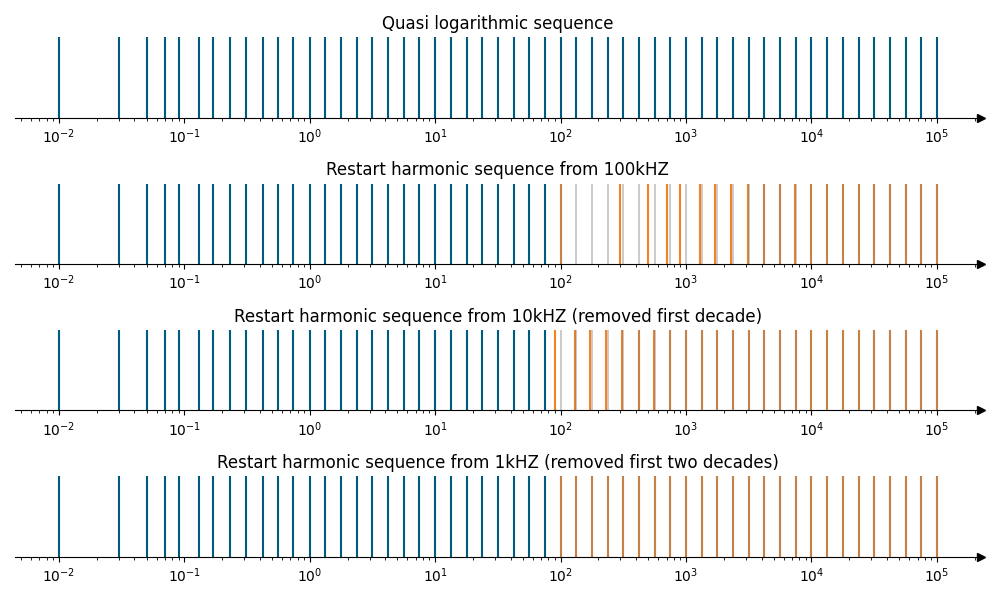
\includegraphics[width=1\linewidth]{figures/harmonics_supporting.png}
    \caption{Enter Caption}
    \label{fig:splitting_design}
\end{figure}
To summarize, for a CCCV experiment for batteries, on channel of the generator would have loaded in memory two low band multisine waves, one optimized for chronoamperometry and the other from chronopotentiometry, and the other channel have loaded the two optimized high band mutisine waves.\\

The automatic switch of the multisine during electrochemical experiments as described before can still be done by DEISchannel for the case of combined multisine waves passing during initialization the object MultisineWaveCombined, also provided  in the package TrueFormAWG.

\subsection{Software}
To streamline the design of multisines I created a Python library also for it, with the name Multisine. It provides the object Multisine that generates multisine, optionally optimize phases for minimal crest factor though iterative randomization and provides tools for visual spectral analysis. It is available as open source software at XXX.github\\

\section{Impedance estimation}
In the experimental works presented in this thesis, we estimated the impedance using the methods of the sliding short-time Fourier transform and dynamic multifrequency analysis; the first only during the online signal processing. The STFFT method has not much tuning. The only user parameters are the length of the window and the windowing function type. The length is dictated by the resolution that one wants to achieve, so on the lowest frequency component of the excitation. The windowing function instead alters the input and output signals time series to put more or less importance to the central part of the signal rather than the borders (makes the impedance confined in time at the price of spectral power) to obtain the instantaneous impedance at the middle points. For the experiment presented here, I assumed that being the drift of the system much slower than the perturbation, the impedance would not vary much and no windowing function is necessary. For the Dynamic Multi-Frequency Analysis, one needs to chose a filter function with care. Here we used the symmetric Fermi-Dirac delta with bandwidth of 0.01 Hz and an order of 8. A previous publication of the group showed the effect of these two parameters on the final result. The most important is the bandwidth because it reflects on the number of spectra estimated and their separation in time. Battistel and al. showed in XX the shape of the filter function when trasnformed to the time domain and it is similar to a sinc function for its main lobe and small oscillation asintothycally to zero. The dynamic multifrequency analysis performes a multiplication in the frequency domain  of the filter with the fourier spectra of the signal around one frequency, that correspond to a convolution of the time domain. Hence the time-domain transformed filter as a function shifted in time by a quantity equal to the reciprocal of the bandwidth. The windows should not be shorter than the period of the multisine and furthermore one should put care in the oscillating lobes that could bias the impedance estimation, as shown in Chukwu.\\

In both methods, one can strongly reduce the zero-frequency skirt in the Fourier space and the Gibbs effect  by removing the baseline for current and voltage signals. I chose to use just a simple baseline removing because other classical methods did not work for me. Typically one can use sliding window averaging, spline or polynomial fitting or gaussian process regression to name the main one. In my experience non of these methods could effectively decouple the trend and the first few frequencies of the multisine that are overlapping. A complete Python library can be used to test these and more trend removal techniques, it is called Wotan. Hellemans and al. developed a method for de-trending signals with low frequency containing multi-sine but there is no available Python implementation to try out and the functional analysis used in the official is above my mathematical skills to implementing it myself.



















\section{Old part}
The estimation of the time-varying impedance require the system to be perturbed with a multi-sine waveform and record input and output synchronously. Most commercial potentiostats-galvanostats do not have the implementation for user-defined arbitrary waveform on the computer user interface to be transferred on the instrument hardware and when a workaround is possible (i.e. ...) the number of points of the multi-sine and the maximum frequency are limited. Usually the buffer memory for the digital-to-analog converter of FPGA boards is a value between 12 kSa and 32 kSa according to my experience browsing manufacturers catalogs, which translates to a multi-sine of ??? decades. Furthermore the maximum frequency of sampling, which defines the maximum recordable tone according to the Nyquist-Shannon theorem, is quite limited due to the difficulty of transferring  big amount of data from the instrument to the computer. The maximum sampling frequency for a premium device might be in the order of 50 kHz. For most electrochemical systems the impedance is informative over 5 or more decades and to frequency up to 1MHz. On the other hand, commercial potentiostats-galvanostats have high precision electronics, with tested circuit boards that allow very small and high current and voltage ranges. The approach used in this work is to integrate a commercial arbitrary waveform generator and a high performance signal acquisition device to a potentiostat/galvanostat exploiting its input and output ports and avoiding the need of designing a high power circuit from scratch. In a nutshell, the set-up we used is composed of an arbitrary waveform generator which applies a custom waveform that define the experiment on the potentiostat though an auxiliary imput. The signal from the cell is recorded on the computer by the digital acquisition device though the auxiliary current and voltage ouput of the potentiostat which sends directly the anaolg signal of the cell. The data are later processed on the computer using custom software.
In the following the parts of the set-up will be better explained, as well as the connection between the devices.

\subsection{Arbitrary waveform generator}
As arbitrary waveform generators we have chosen the TrueForm 33500B series because of its elevate digital-to-analog converter memory buffer. Two models has been used, the 33520B and 33522B which differs only in the value of buffer memory, the first of 16MSa and the second of 64MSa, both per channel. The other important characteristic of these devices are
\marginpar{
\centering
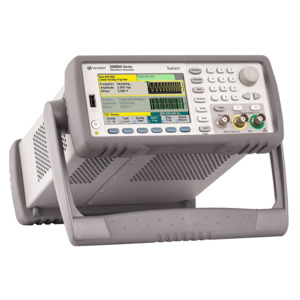
\includegraphics[width = 0.95\marginparwidth]{figures/truform_white.jpg}
%\captionof{figure}{Arbitrary waveform generator Keysight Trueform 33520B}
Model 33520B
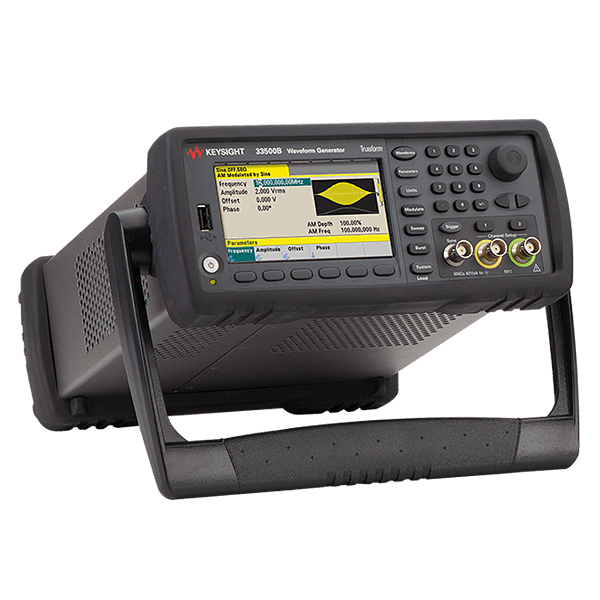
\includegraphics[width = 0.95\marginparwidth]{figures/truform_black.png}
Model 33522B
\captionof{figure}{Keysight Trueform arbitrary waveform generator units from the series 33500.}
\label{fig:awg photo}
}
\begin{itemize}
    \item high frequency generation capability of 20MHz, much higher then the electrochemical upper response limit (usully below 1MHz),
    \item two distinct channels with own memory and the possibility to store multiple waveforms,
    \item possibility to sum the waveform in the two channels (and output the total on channel 1),
    \item imrpoved signal integrity thanks to high generation fidelity with 0.03\% of harmonic distortion, a jitter as low as 1 ps and proprietary \emph{Trueform} generation technology compared to the Direct Digital Synthesis method; all contributes to reduce any source of intermodulation in the multisine. \\ (more on that \url{https://www.youtube.com/watch?v=HLPoSiorh30})
\end{itemize}
Further details are reported in the witepapers supplied by the company Keysight though their website.

The user can set the parameters using the convenient front panel of the device, as shown in Figure \ref{fig:awg photo} or sending commands via USB or Ethernet connection. The instrument can communicate with a computer through SCIPI (Standard Commands for Programmable Instruments) language. I developed a small but convenient Python module to communicate with the instrument using the PyVISA package, Python implementation of VISA (Virtual Instrument Software Architecture). The module is available on my GitHub page (\url{https://github.com/federicoscarpioni/TrueFormAWG}). The manufacturer also provides a collection of stand-alone software for the control of the instruments, the design of  waveforms and automation of electrical tests, that I did not used for this work. An exception is the software Keysight connect to verify the connection with the instrument through USB or Ethernet sub-network and get their addresses for establishing the connection with the dedicated Python library mentioned before.

\section{Multi-sine design}

\subsection{Running the multi-sine in the waveform generator}
The waveform can be transferred via USB drive accessing the front panel or via SCIPI communication.


\subsection{Digital acquisition device}

The acquisition stage of the set-up must satisfy two requirements:
\begin{itemize}
    \item Sampling at frequency of the order of MHz,
    \item Sample very long signals of hundreds of thousands of points.
\end{itemize}
Many solutions are available on the market to easily achieve these goals. They mainly fold into two categories base on their connection: USB or PCI. For this work we chose to use a USB device which satisfies all the requirements while being relatively inexpensive. USB devices are practical and portable and it is possible to connect many of them on the same computer. The devices chosen are from the PicoScope digital computer oscilloscope from Pico Technology. The devices can interface with a computer through the proprietary software PicoScope Software or the feature-rich software development kit available in multiple programming languages directly from the manufacturer GitHub page (\url{https://github.com/picotech}). Pico Technologies sells different series of devices with different capabilities. In this work we used 
\begin{itemize}
    \item PicoScope 4824A (4000A series) with 8 channles and a resolution of 12bit,
    \item PicoScope 4262 (4000 series) with 2 channles and a resolution of 16bit,
    \item PicoScope 5442D (5000 seires) with 4 channels and a resolution of 16-15-14 or lower bit depending on the number of channels active.
\end{itemize}
For the concerns of this work, the main differences between the devicea are
\begin{itemize}
    \item the number of channels,
    \item the resolution of the analog-to-digital converter expressed in bit (higher number is better, as discussed in \ref{sec:ADC})
    \item the maximum sampling frequency (which is always fare above the needs in electrochemistry),
    \item the cutting frequency of an internal filter low-pass filter.
\end{itemize}
The peculiar characteristics of these devices is the \emph{streaming mode} for transferring continuous acquisition of signals without loss even when the signal is longer than the device memory (other modes are available such as block mode and ???). 
The software development kit (SDK) from the manifacturer provides an interface to the USB drivers to conveniently include the streaming of data into the user program. The streaming mode works as follow: the user defines in their program a memory segment and a function to execute some actions on the data which are bidden to the software and when some new data is ready, the USB drive automatically writes the new numbers in the memory segment and calls the function (which is commonly referred to as callback function). In the callback the data in the memory segment should be processed, saved or evaluated in some way because will be overwritten in the next call anyway.
The routine runs in a infinite \lstinline[language=Python]{while} loop.
A common approach, and also the suggestion from the manual, is to have another memory segment in the user program, let's call it \emph{signal storage} for clarity despite being save on the RAM volatile memory and not in the permanent disk, large as much as the signal to sample where to copy the new data at each execution of the callback. The manual from the manufacturer gives a lot of information on the streaming mode and how to set it up. Code examples are also available for each supported programming language.

The data streamed are the numbers coming from the digitization step and they need to be converted before using them. The conversion factor depends on the resolution of the devices used (see \ref{sec:ADC}).

The most streighforward to handle the streaming data is to keep in memory all the data coming from the devices and then save the data to storage. This is the approach used also for this work at the beginning. The limitation is the actual RAM memory installed in the computer in use. A standard office computer with 16 GB of RAM might be sufficient to store the complete voltage and current signals for short measurements. The duration of such experiment would depend on the aquisition frequency. The ammount of points that can be usually stored in 16GB is 900.000.000 per channel which correspond to ?? GB . The memory occupied by the operating system and other application has to be taken into account. For example, when acquiring at 5MHz with the PicoScope the acquisition lasts 180 seconds while at 5KHz 50 hours. The first case should apply for studying electrode reactions during voltage sweep technique as for the study of hydrogen evolution on catalysts while the second for the study of battery degradation in galvanostatic mode. 50 hours is still a short time when compared to Li-ion batteries that it in the order of month. To measure the impedance for such long time one might decide to periodically store data into the computer hard-drive freeing up the memory or acquiring the signals not for every cycle. This ideas will be further development in a later paragraph.




\section{Connecting cells in three-electrode configuration}
Collecting the time-varying impedance of both positive and negative electrode of a three-electrode cells together requires some considerations. The potentiostats/galvanostats have usually only two auxiliary analog outputs: voltage versus reference and current. Furthermore, in any technique, the device controls the voltage difference between working and reference terminal. It effects either chrono-amperometric techniques because the counter as traditional for electrochemistry is only there to complete the circuit and chrono-potentiometric were despite the controlled counter being the same in the entire cell, it is not always possible to control the full cell voltage as it is not output in analog signal. Biologic devices are capable of changing the voltage control from working electrode vs reference to working vs counter through the hardware configuration section of the software EC-Lab. Unfortunatly this is not implemented in the EC-Lab SDK version ?? and one must come up with alternative, creative solutions. The easiest workaround is to employ two channels of the potentiostat, both in two electrode configuration with on to controll the techniques between working and counter electrode and the other between working and reference electrode to record the voltage drop in the half cell in OCV technique. 
Using just one channel of the instrument in three-electrode configuration and measure the voltage between working and counter (the full cell volage) with the digital aquisition device doesn't allow the controll of the full cell voltage, which is crucial for batteries, and connecting the instrument in two electrode configuraion connecting working and counter and recoridng the voltage drop between working and reference is not a good practice because the imput impedace of the PicoScope is just of 10 MOhm, one order of magniuted less than a potentiostat, that would cause a big bias current flowing on the referenece drifting it out of the quasi-thermodynamic equilibrium that would have instead.

\section{Electrochemical devices}
For these work we decided to use BioLogic potentiostats/galvanostats from the Premium class which can work easily with external connection using the EC-Lab software (from version ??? or EC-Lab express all versions). The devices used for this work are:
\begin{itemize}
    \item SP-300 two channels,
    \item VSP-3 six channels,
\end{itemize}
fully equiped with Frequency Response Analyzer for measring the impedance up to 1MHz. The voltage range span between -12 and 12V, the total current across the channels is of 500mA, many current ranges are availabel and the analog to digital converter resolution is of 16 bit. These devices are configured with the EC-Lab and EC-Lab Express software. A software Development Kit for EC-Lab is also available in different programming languages albeit not officially supported by the manufacturer.
In addition, for less demanding circumstance, a BioLogic battery cycler ??? was used



\section{Connecting the device and acquiring the signals: set-up version 1}
In the previous section, it was discussed how it is possible to generate and acquire multi-frequency signals. Now it is time to dig into the combination of these device for create a set-up suitable for the measurement of impedance in non-stationary conditions. The central point of such set-up is the potentiostat/galvanostat that provides all the electronics and implementation of electrochemical techniques. Some of the commercial devices have the ability to receive and record external signals or output directly the analog signals for voltage and current though coaxial connector. 

\section{Automatic cycling with}